\chapter{РЕЗУЛЬТАТЫ}
\label{ch:РЕЗУЛЬТАТЫ}

В этой главе описываются оценочные тесты, выполненные для проверки предложенного подхода на основе разработанного фреймворка. Следующие разделы предназначены для предоставления информации о подготовке исходных данных, представления и обсуждения полученных результатов. Сначала будет рассмотрена аппроксимация траекторий с использованием полиномиальной регрессии. Далее будет проведена провека точности результирующих кластеров точность с использованием вышеупомянутого индекса DI. Глава завершается обсуждением выходных результатов этапа классификации и демонстрацией результатов проверки качества обнаружения аномалий.

\section{Оценка точности}

В этом разделе подробно описываются подготовка и результаты оценочных тестов, выполненных для проверки точности, достоверности полученных результатов.

\subsection{Результаты аппроксимации траекторий}

Для того чтобы принять решение о степени полиномов для аппроксимации, было проведено несколько экспериментов. Были предприняты попытки аппроксимировать исходные траектории полиномами $3$-ей, $4$-ой, $5$-ой степеней соответственно. В следующей таблице приведены минимальные и средние значения коэффициента детерминации $R^2$ для каждого из экспериментов (табл. \ref{table:r2_res}).

\begin{table}[h!]
	\caption{Значения коэффициента $R^2$ для полиномов различных степеней}
	\label{table:r2_res}
	
	\setlength{\tabcolsep}{10pt}
	\centering
	\begin{tabular}[c]{|| C{2cm} | C{2cm} C{2cm} | C{2cm} C{2cm} ||} 
		\hline
		\multirow{3}{7em}{Degrees of polynomials} 	& \multicolumn{4}{c||}{$R^2$ score} \\[1ex]\cline{2-5}
		& \multicolumn{2}{c|}{X}	& \multicolumn{2}{c||}{Y} \\ [0.5ex]
		& min 	& avg				& min 	& avg \\ [0.5ex]
		\hline \hline
		\rowcolor{nogray} \multicolumn{5}{||c||}{$1.txt$ (before filtering)} \\ [0.5ex]
		\hline
		\{3\} 							& 0.66 	& 0.994 & 0.466 & 0.989 \\ [2ex]
		\rowcolor{backgray} \{3, 4\} 	& 0.897 & 0.998 & 0.823 & 0.994 \\ [2ex]
		\{3, 4, 5\} 					& 0.949 & 0.998 & 0.864 & 0.995 \\ [2ex]
		
		\hline \hline
		\rowcolor{nogray} \multicolumn{5}{||c||}{$1.txt$} \\ [0.5ex]
		\hline
		\{3\} 							& 0.689 & 0.997 & 0.777 & 0.995 \\ [2ex]
		\rowcolor{backgray} \{3, 4\} 	& 0.942 & 0.999 & 0.872 & 0.997 \\ [2ex]
		\{3, 4, 5\} 					& 0.98 	& 0.999 & 0.88 	& 0.997 \\ [2ex]
		
		\hline \hline
		\rowcolor{nogray} \multicolumn{5}{||c||}{$2.txt$} \\ [0.5ex]
		\hline
		\{3, 4\} 						& 0.992 & 0.9997 & 0.832 & 0.996 \\ [2ex]
		\hline \hline
		
		\rowcolor{nogray} \multicolumn{5}{||c||}{$3.txt$} \\ [0.5ex]
		\hline
		\{3, 4\} 						& 0.815 & 0.995 & 0.867 & 0.996 \\ [2ex]
		\hline \hline
		
		\rowcolor{nogray} \multicolumn{5}{||c||}{$4.txt$} \\ [0.5ex]
		\hline
		\{3, 4\} 						& 0.879 & 0.995 & 0.722 & 0.993 \\ [2ex]
		\hline
	\end{tabular}
\end{table}

В этом параграфе будет приведено обсуждение результатов экспериментов на примере траекторий с первого перекрестка ($ 1.txt $) до и после фильтрации траекторий. Из табл. \ref{table:r2_res} видно, что средние значения коэффициента $R^2$ приемлемы для всех экспериментов. Однако минимальные значения $R^2$, которые равны 0,66 и 0,466 для первого эксперимента с полиномами только $3$-ей степени для неотфильтрованных траекторий являются неудовлетворительными, что означает, что модель может корректно предсказать только половину всех точек траекторий. Фильтрация и игнорирование коротких траекторий с малым итоговым пространственным смещением значительно улучшили результаты. Однако результаты для аппроксимации с использованием полиномов $3$-ей степени все еще неудовлетворительны. Это может повлиять на последующий анализ и ухудшить дальнейший анализ. По этой причине было выполнено приближение с использованием полиномов различных степеней одновременно следующим образом:

\begin{enumerate}
	\item сначала выполнить аппроксимацию, используя низшую степень полинома в качестве отправной точки,
	\item сравнить полученные значения коэффициента детерминации $R^2$ с заранее заданным граничным значением (0,98 в данном случае); если полученное значение меньше предопределенного порога, увеличить ожидаемую степень полинома и выполнить полиномиальную регрессию снова,
	\item продолжать увеличивать степень полинома до получения приемлемых значений $R^2$ или до достижения заданного ограничения максимальной допустимой степени полинома (5 в данном случае). 
\end{enumerate} 

Аппроксимация полиномами $3$-ей и $4$-ой степеней в совокупности значительно улучшила как минимальные, так и средние значения $R^2$. Однако добавление полинома $5$-ой степени не оказало существенного влияния на результаты и улучшило средний коэффициент только на 0,01 по сравнению с предыдущим экспериментом. В связи с этим было решено сосредоточиться на приближении с использованием полиномиальных функций $3$-ей и $4$-ой степеней и провести эксперименты на траекториях с других перекрестков ($2.txt$, $3.txt$, $4.txt$).

Для упрощения повествования траектории будут классифицированы на две группы в зависимости от степени полиномов, использованных для аппроксимации: первая группа включает в себя траектории, аппроксимированные полиномиальными функциями $3$-ей степени, в то время как вторая группа состоит из траекторий, аппроксимируемых полиномами $4$-ой степени. Траектории обеих групп были проанализированы с точки зрения формы и средней скорости. На рис. \ref{fig:regr-pol-4} показана вторая группа траекторий, а в табл. \ref{table:speeds} указаны представлены минимальная, средняя и максимальная скорости траекторий для обеих групп.

\begin{figure}
	\centering
	\begin{subfigure}[b]{0.3\textwidth}
		\centering{}
		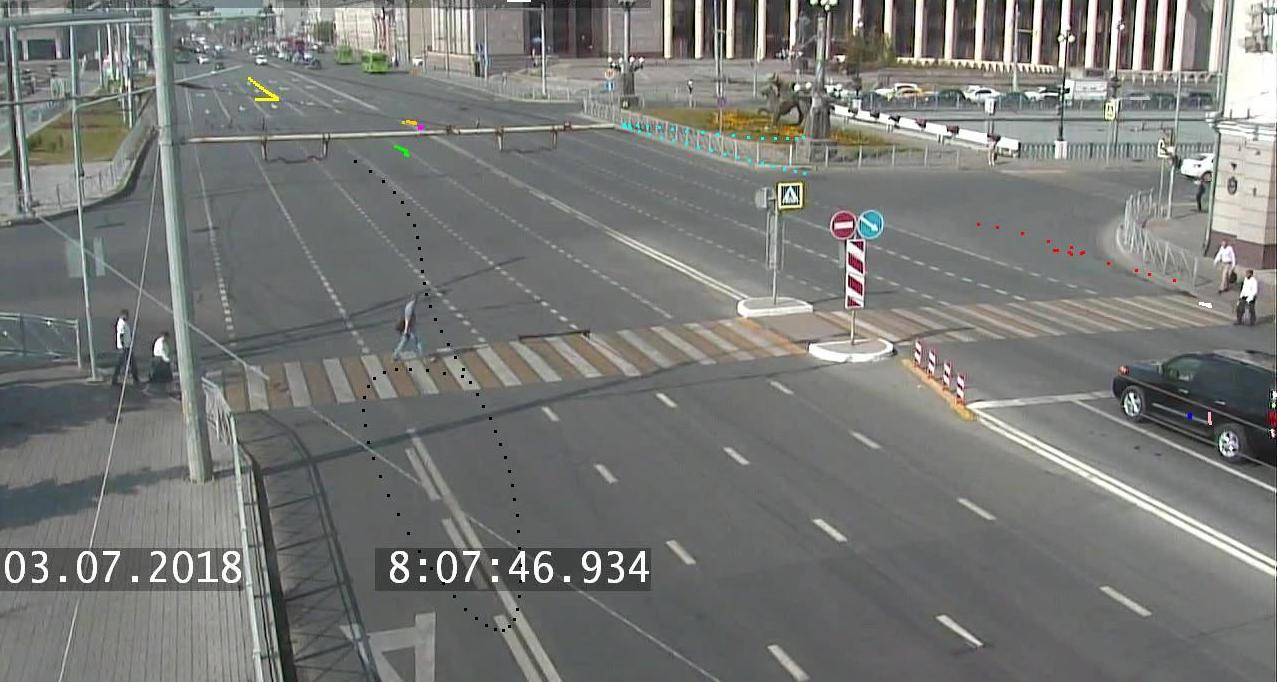
\includegraphics[width=\textwidth]{images/regr_1_pol_4.jpg}
		\caption{$1.txt$}
		\label{fig:regr-1-pol-4}
	\end{subfigure}
	\hfill
	\begin{subfigure}[b]{0.3\textwidth}
		\centering{}
		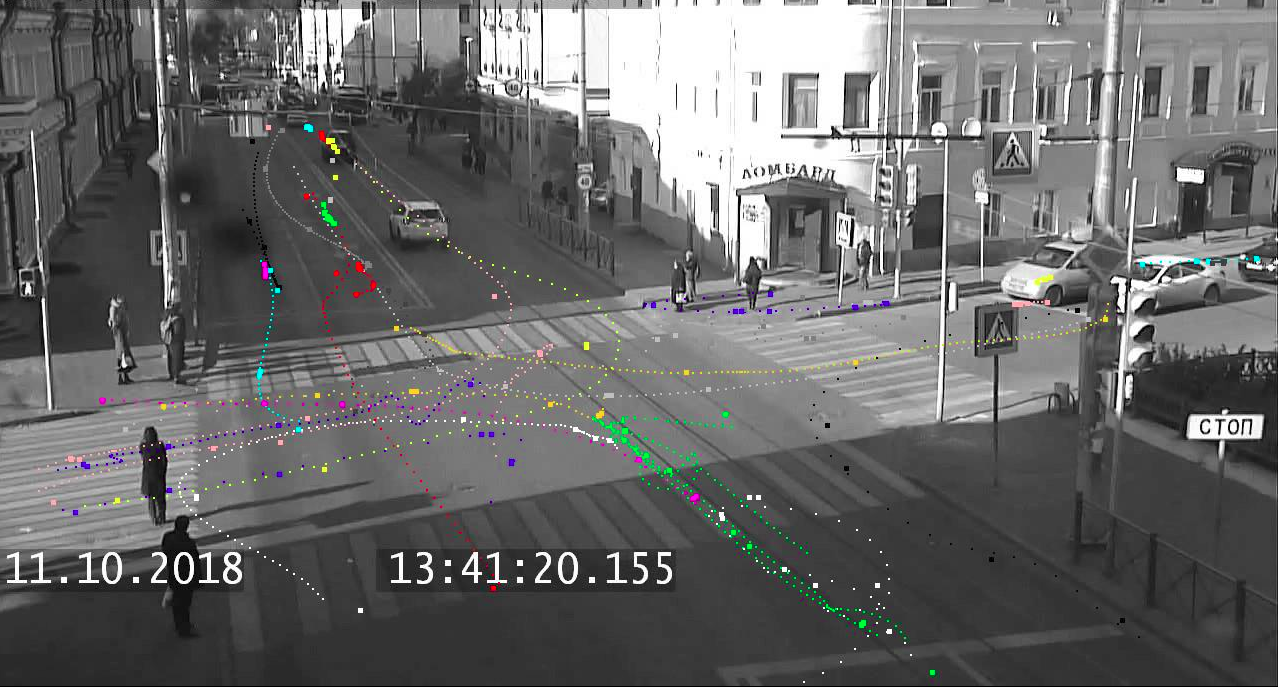
\includegraphics[width=\textwidth]{images/regr_3_pol_4.png}
		\caption{$3.txt$}
		\label{fig:regr-3-pol-4}
	\end{subfigure}
	\hfill
	\begin{subfigure}[b]{0.3\textwidth}
		\centering{}
		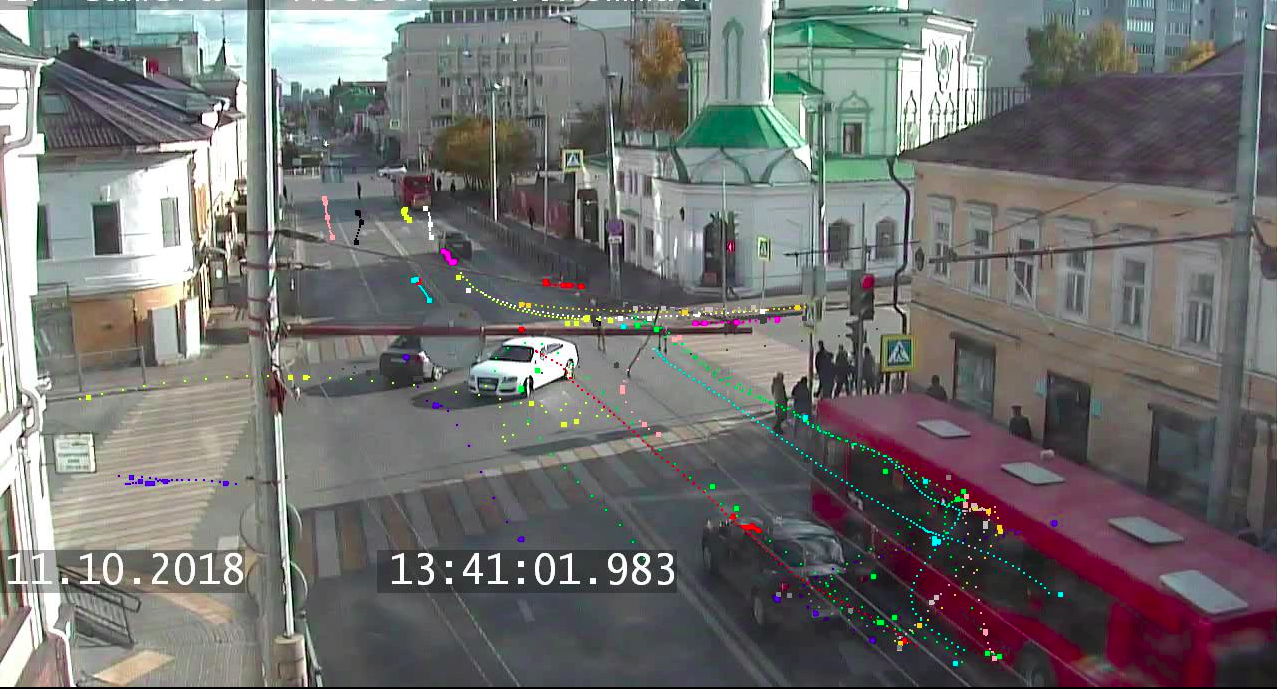
\includegraphics[width=\textwidth]{images/regr_4_pol_4.png}
		\caption{$4.txt$}
		\label{fig:regr-4-pol-4}
	\end{subfigure}
	\caption{Траектории, аппроксимированные полиномами $4$-ой степени}
	\label{fig:regr-pol-4}
\end{figure}

\begin{table}[h!]
	\caption{Сравнение минимальной, средней, максимальной скоростей ТС}
	\label{table:speeds}
	
	\setlength{\tabcolsep}{10pt}
	\centering
	\begin{tabular}[c]{|| C{2.5cm} | C{2.5cm} C{2.5cm} C{2.5cm} ||} 
		\hline
		\multirow{2}{7em}{Degree of a polynomial} 	
		& \multicolumn{3}{c||}{Speed \textit{(pixels per sec)}} \\[1ex]\cline{2-4}
		& min 		& avg		& max 				\\ [2ex]
		
		\hline \hline
		\rowcolor{nogray} \multicolumn{4}{||c||}{$1.txt$ (before filtering)} 	\\ [0.5ex]
		\hline
		\rowcolor{backgray} \{3\} 	& 18.555 	& 335.365 	& 1721.499 			\\ [2ex]
		
		\rowcolor{backgray} \{4\} 	& 1.206		& 72.34 	& 374.396 			\\ [2ex]
		\hline
		
		\rowcolor{nogray} \multicolumn{4}{||c||}{$1.txt$} 	\\ [0.5ex]
		\hline
		\rowcolor{backgray} \{3\} 	& 61.814 	& 372.435 	& 909.121 			\\ [2ex]
		
		\rowcolor{backgray} \{4\} 	& 26.603	& 229.053 	& 602.773 			\\ [2ex]
		
		\hline
		\rowcolor{nogray} \multicolumn{4}{||c||}{$2.txt$} 	\\ [0.5ex]
		\hline
		\{3\} 	& 85.705 	& 494.016 	& 1107.96 			\\ [2ex]
		
		\{4\} 	& 183.087	& 613.865 	& 900.737 			\\ [2ex]
		\hline
		
		\rowcolor{nogray} \multicolumn{4}{||c||}{$3.txt$} 	\\ [0.5ex]
		\hline
		\{3\} 	& 13.65 	& 301.481 	& 1012.748 			\\ [2ex]
		
		\{4\} 	& 29.26		& 206.119 	& 764.25 			\\ [2ex]
		\hline
		
		\rowcolor{nogray} \multicolumn{4}{||c||}{$4.txt$} 	\\ [0.5ex]
		\hline
		\{3\} 	& 43.01 	& 269.074 	& 872.33	 		\\ [2ex]
		
		\{4\} 	& 22.92		& 163.431 	& 708.154 			\\ [2ex]
		\hline
		
	\end{tabular}
\end{table}

Далее траектории, аппроксимированные полиномами $3$-ей $4$-ой степеней будут обозначаться первой и второй группами траекторий соответственно. Можно заметить, что траектории из разных групп имеют очень разные скорости. Первая группа включает в себя траектории с гораздо более высокими скоростями, особенно выделяется, что максимальная скорость для второй группы почти равна средней скорости для первой группы, а средняя скорость для первой группы почти в четыре раза больше, чем для второй группы для случая неотфильтрованных траекторий. После исключения коротких траекторий из рассмотрения результаты стали более плавными, однако те же наблюдения и выводы имеют место быть. Также на рис. \ref{fig:regr-pol-4} видно, что полиномиальные функции 4-го порядка использовались для аппроксимации траекторий более сложной формы или траекторий с плотно расположенными точками траектории.

Такая тенденция в основном различима при рассмотрении траекторий с первого перекрестка. Данные с первого перекрестка могут считаться репрезентативным набором траекторий, поскольку он имеет наибольшее количество экземпляров данных. Также стоит отметить, что второй набор данных траекторий ($2.txt$) имеет только 10 траекторий в первой группе, поэтому анализ скорости траекторий не может быть очень точным.

\subsubsection{Выводы}

Таким образом, из вышеизложенных результатов следует, что полиномиальные функции высшего порядка предпочтительнее для аппроксимации траекторий следующих групп:

\begin{itemize}
	\item траектории медленно движущихся или неактивных ТС (включая траектории ТС, ожидающих на перекрестках на светофоре), которые продемонстрированы на \ref{fig:regr-1-pol-4};
	\item траектории ТС, движущихся с непостоянной скоростью или ускорением на некоторых участках траектории (могут быть представлены неравным распределением точек траектории, где плотные области точек траектории сигнализируют об ускорении в течение этих временных интервалов; как результат, полиномы низкого порядка не могут описать такую сложную зависимость между пространственной координатой и временем);
	\item траектории сложной формы (резкие повороты, улитки Паскаля), особенно различимо на рис. \ref{fig:regr-pol-4}b-c.
\end{itemize}

\subsection{Результаты кластеризации траекторий}

Было проведено 2 эксперимента на одном и том же наборе данных ($2.txt$) с разным числом итоговых кластеров: 8 и 9. Согласно результатам экспериментов, объединение до 8 кластеров продемонстрировало более точное разбиение данных и более высокие значения DI. Результаты выполнения кластеризации на примере данных с первого перекрестка представлены на рис. \ref{fig:clust-res}, кластеры данных обозначены различными цветами. На рис. \ref{fig:9cl-di-94} видно, что возможно и желательно дальнейшее объединение кластеров, представленных желтым и зеленым цветами. Рис. \ref{fig:8cl-di-95} демонстрирует результат продолжения кластеризации (в данном случае объединения кластеров), в котором два указанных кластера объединены в один на основании малого значения расстояния между ними (высокой степени схожести).

\begin{figure}[!htb]
	\centering
	\begin{subfigure}[!htb]{0.8\textwidth}
		\centering{}
		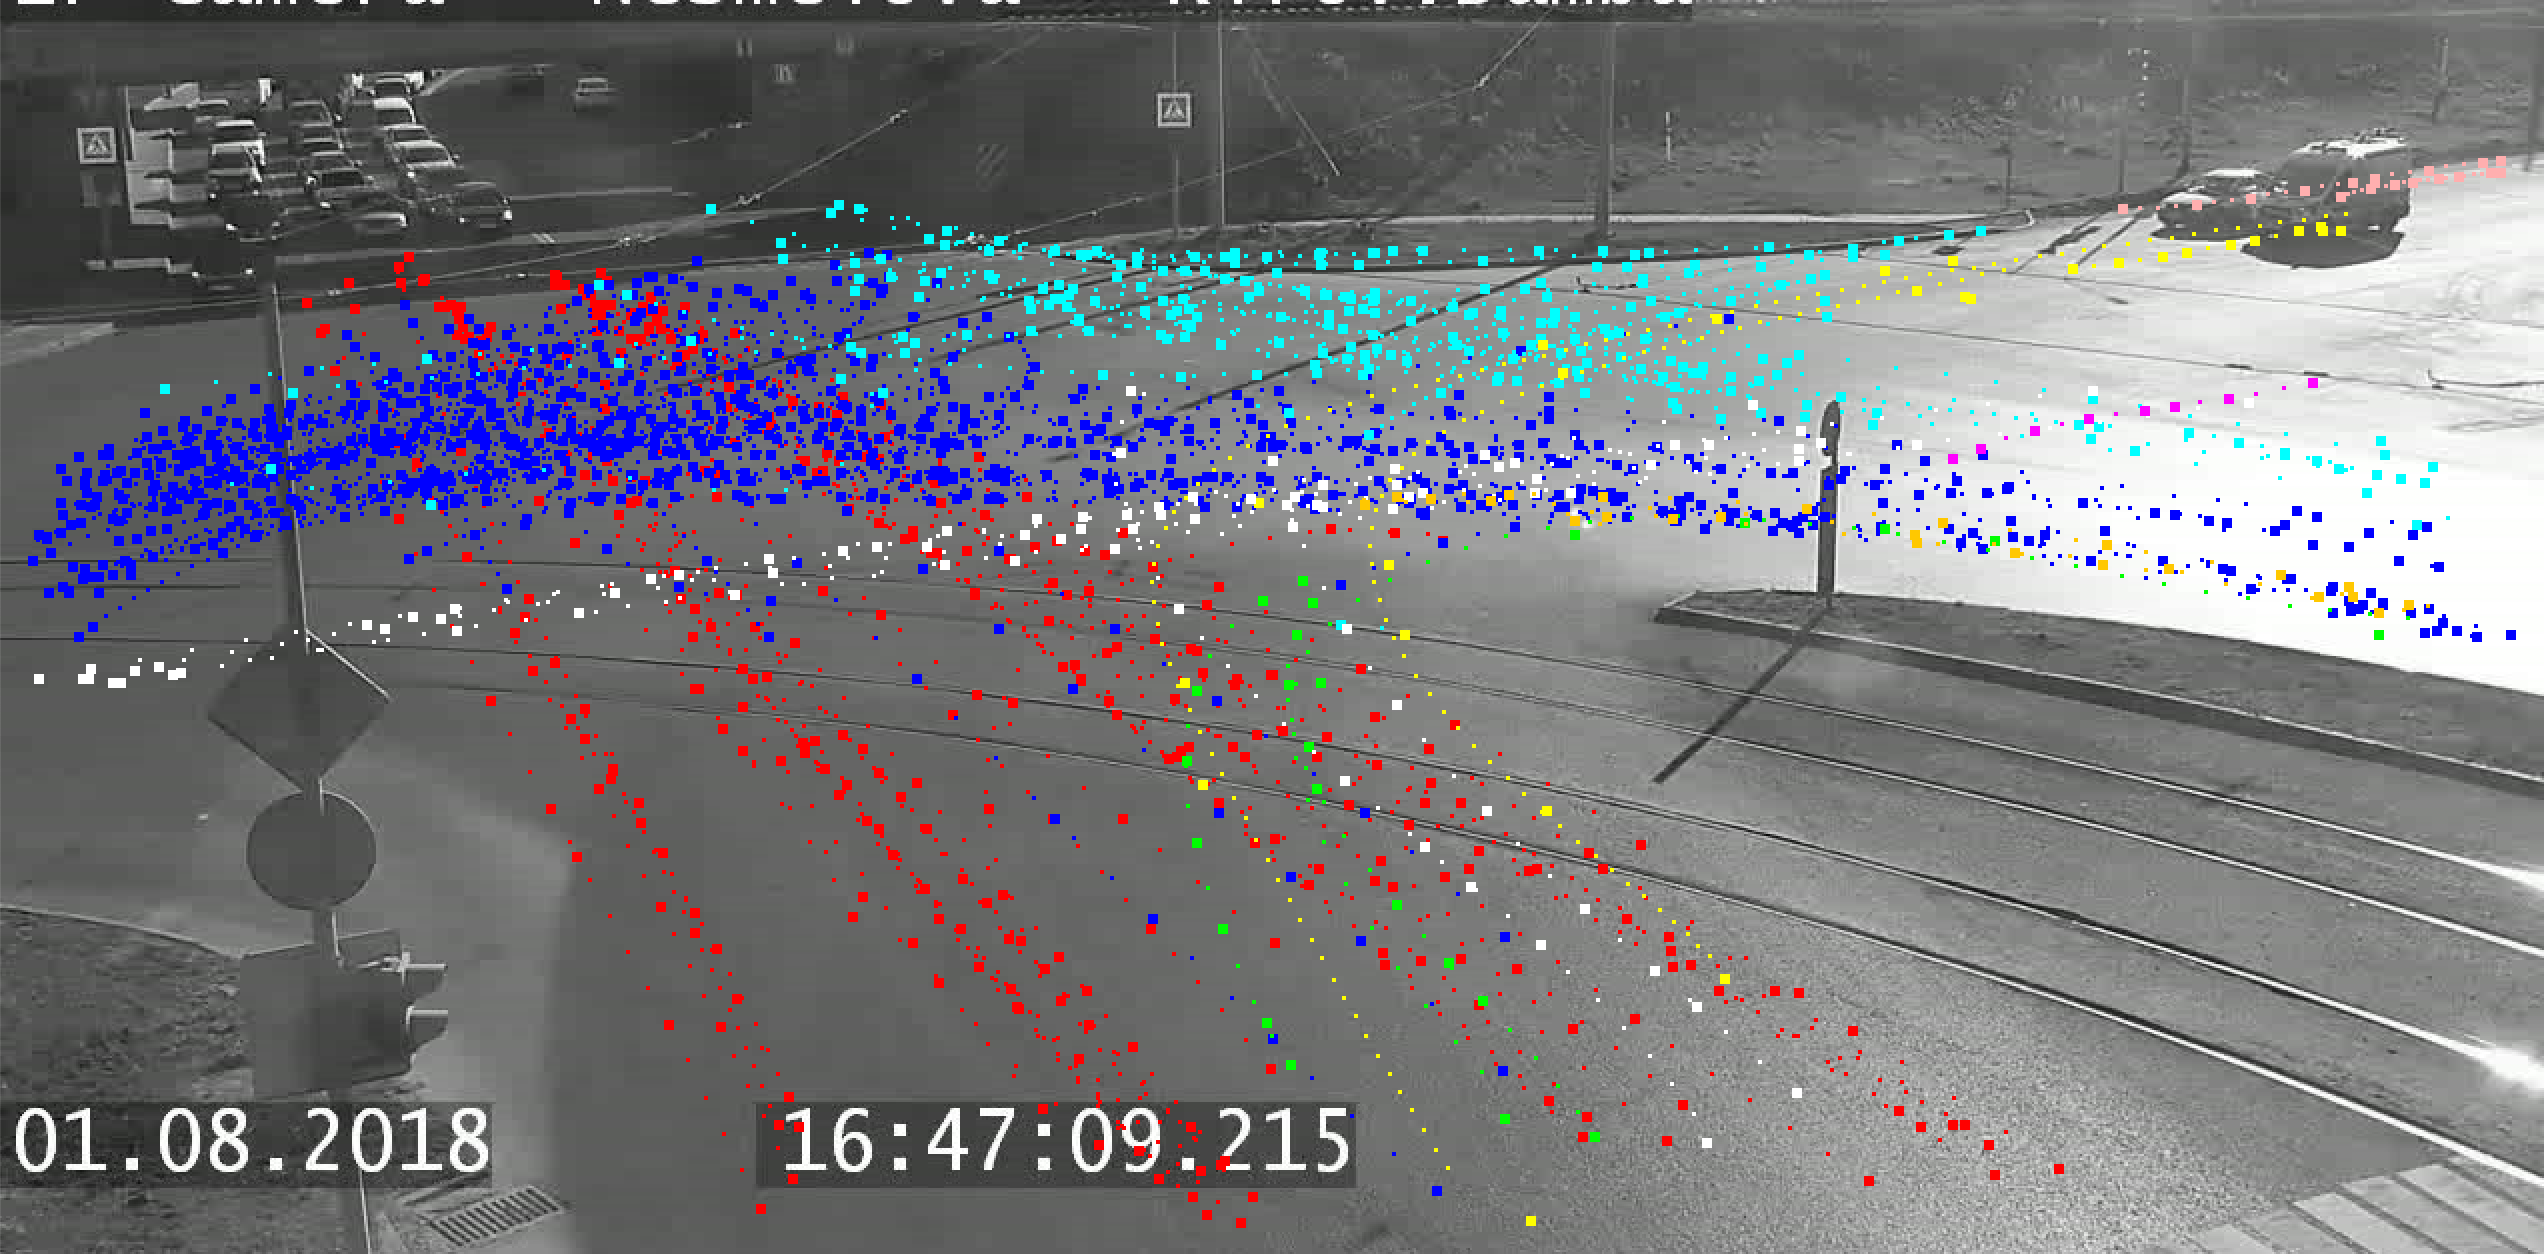
\includegraphics[width=\textwidth]{images/9cl-di-94.png}
		\caption{9 итоговых кластеров, DI = 0.94}
		\label{fig:9cl-di-94}
	\end{subfigure}
	\hfill
	\begin{subfigure}[!htb]{0.8\textwidth}
		\centering{}
		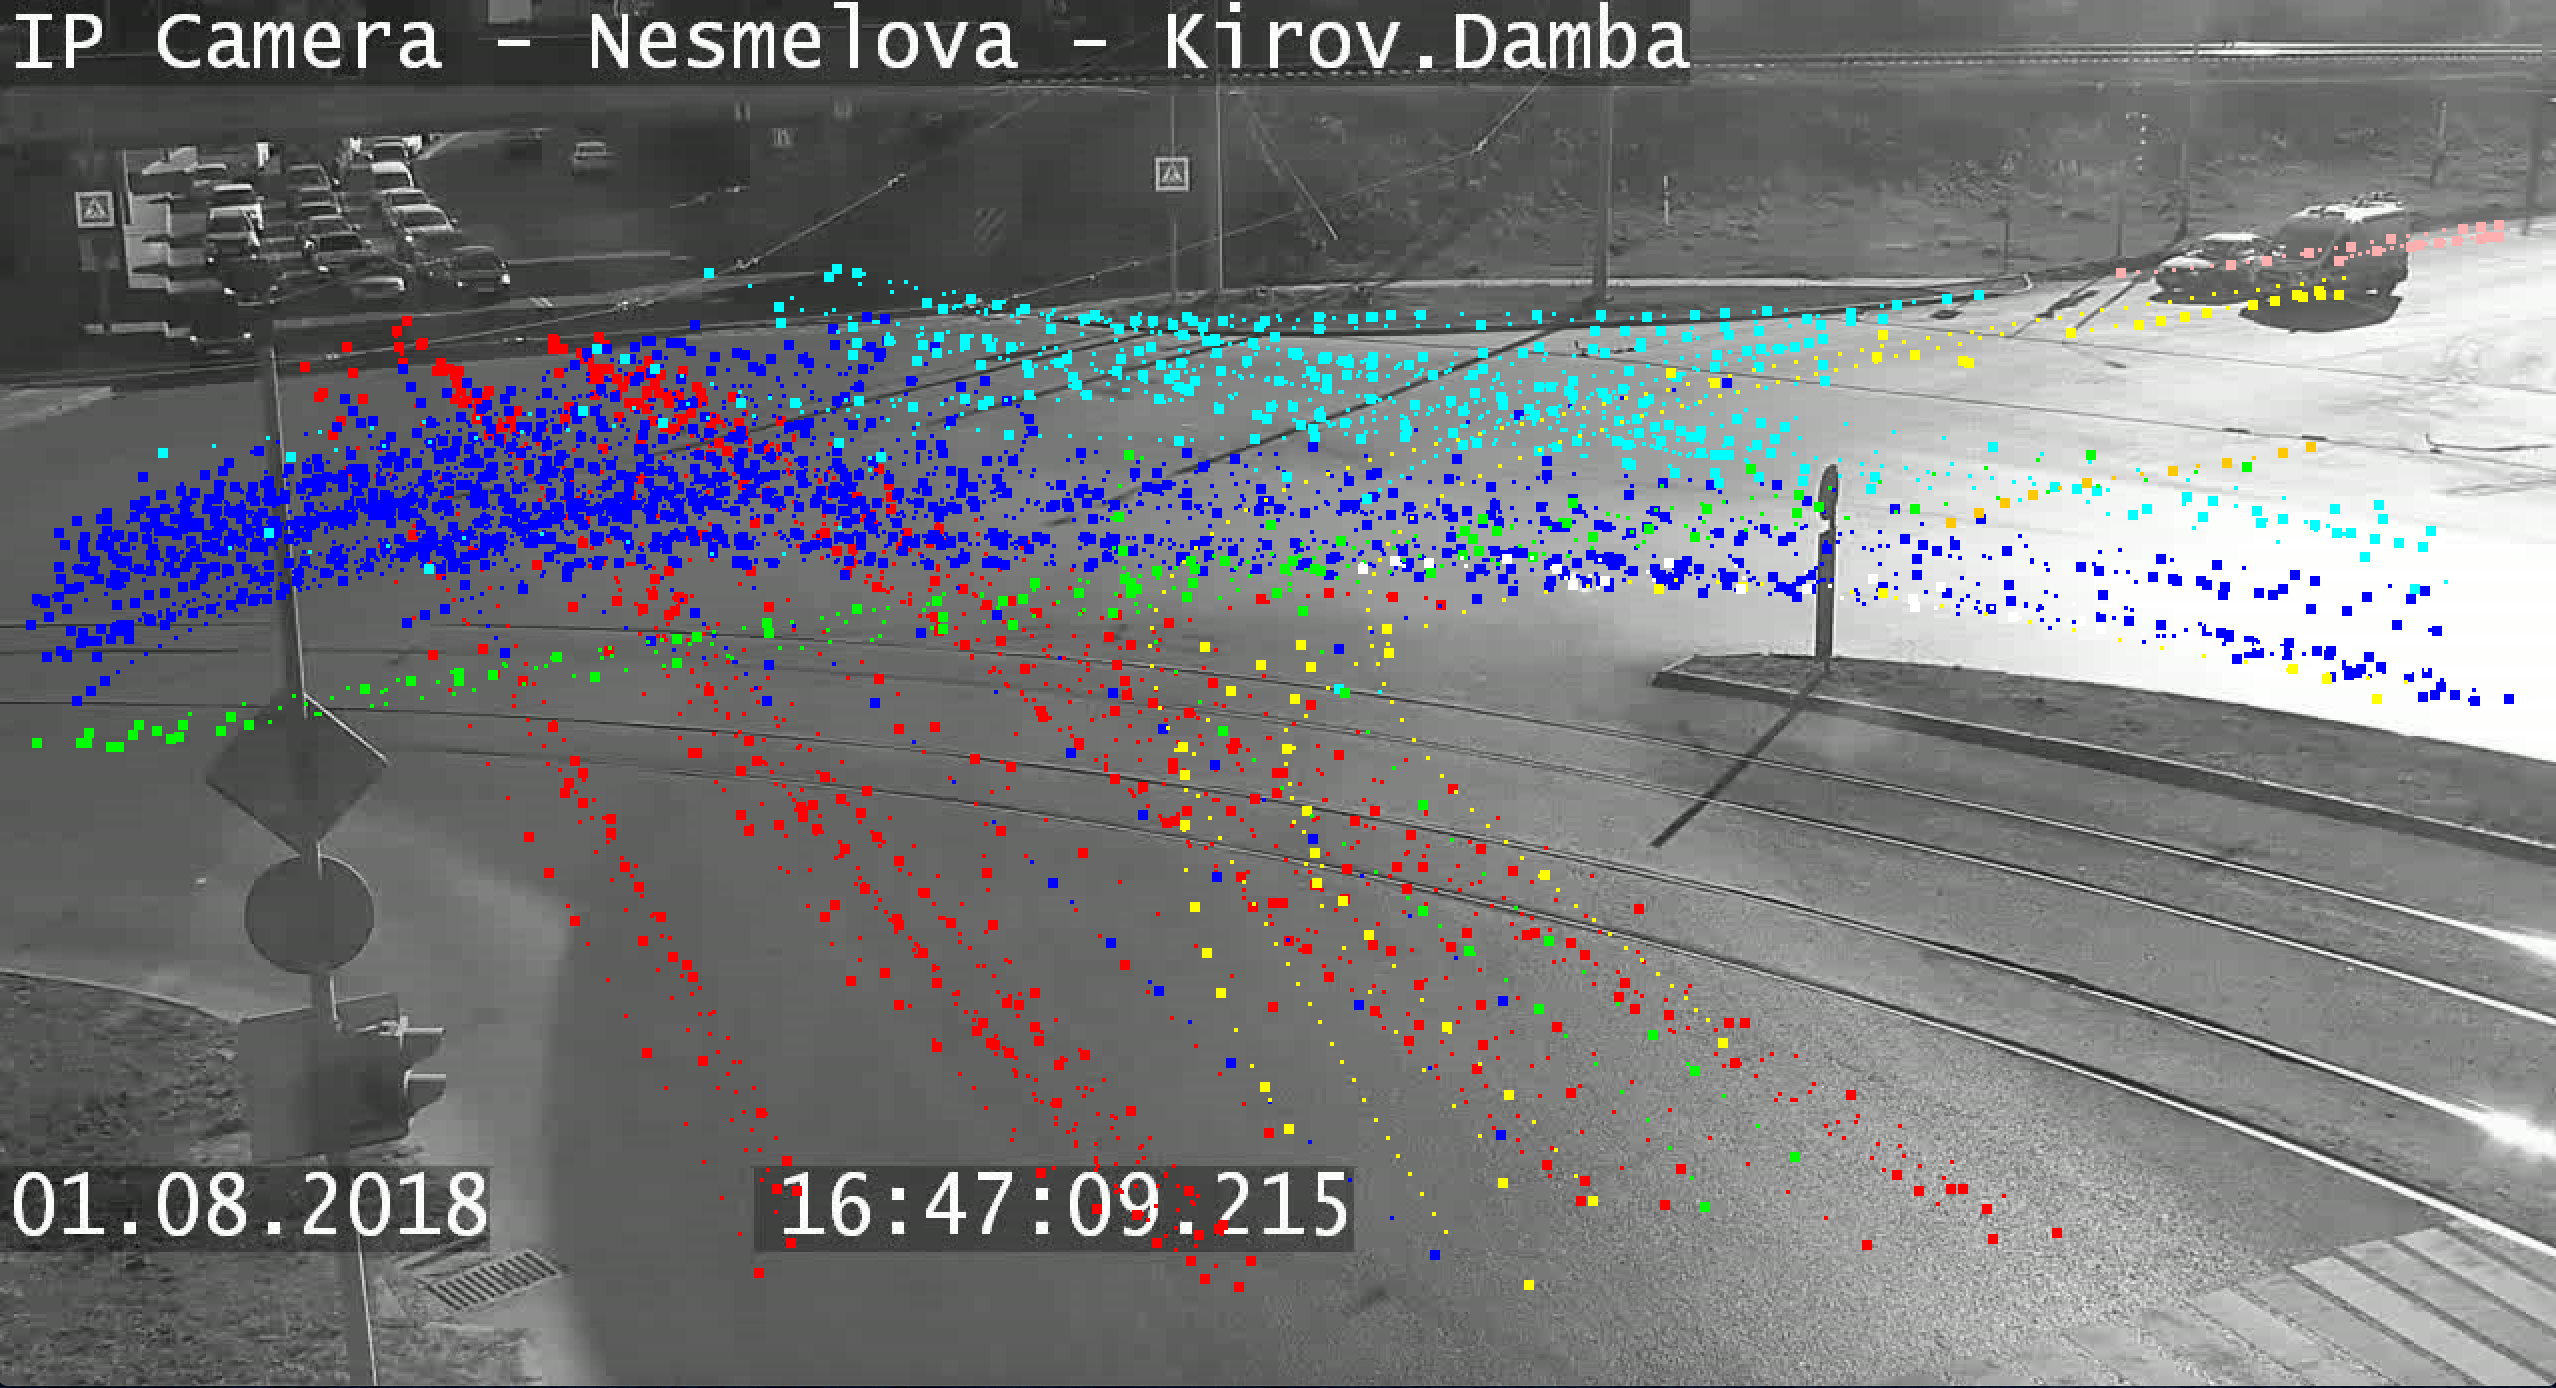
\includegraphics[width=\textwidth]{images/8cl-di-95.png}
		\caption{8 итоговых кластеров, DI = 0.95}
		\label{fig:8cl-di-95}
	\end{subfigure}
	\caption{Результаты кластеризации на примере траекторий со второго перекрестка}
	\label{fig:clust-res}
\end{figure}

Валидация полученных кластеров была проведена с использованием метрики DI, были получены следующие значения:
\begin{itemize}
	\item 9 кластеров -- DI = 0.94,
	\item 8 кластеров -- DI = 0.95.
\end{itemize}

Однако, несмотря на высокое значение DI, можно заметить, что результат кластеризации содержит ошибки: синие ключевые точки, соответствующие синему кластеру траекторий, накладываются на траектории красного кластера. Возможной причиной такого поведения является высокая степень сходства между этими траекториями и другими траекториями синего кластера в левой верхней половине рисунка: эта область представлена густым скоплением точек синего цвета.

При подсчете метрики LCSS для кластеризации были реализованы адаптивные параметры $\delta$ и $\varepsilon$. В качестве функциональной зависимости между параметров $\varepsilon$ и расстоянием между точкой траектории и камеры были выбраны следующие отношения:

\begin{equation} \label{eq:delta-adapt}
	\delta = coeff * \min{(t1.length(), t2.length())}
\end{equation}

\begin{equation} \label{eq:epsilonX-adapt}
\varepsilon_x = coeff * (maxX - minX) / distanceToCamera
\end{equation}

\begin{equation} \label{eq:epsilonY-adapt}
\varepsilon_y = coeff * (maxY - minY) / distanceToCamera
\end{equation}

где $distanceToCamera$ вычисляется как Евклидово расстояние между данной точкой траектории и точкой местоположения камеры на текущем перекрестке, а $coeff$ - коэффициент, значение которого будет подобрано экспериментальным путем. В данном случае наилучшие результаты были получены для значения коэффициента $coeff = 20.0$ и статистика средних и минимальных значений адаптивных $\varepsilon$ для каждой из осей представлены ниже:

\begin{tabular}{lllll}
	\multicolumn{5}{c}{\bm{$\varepsilon$}}\\
	$X:$       			& & & \\[0.5ex]
						& max 	& = 	& 351.397 	& (pixels) \\[0.5ex]
						& min 	& = 	& 23.248 	& (pixels) \\[0.5ex]
	$Y:$       			& & & \\[0.5ex]
						& max 	& = 	& 151.252 	& (pixels) \\[0.5ex]
						& min 	& = 	& 10.004 	& (pixels) \\[0.5ex]

\end{tabular}

\subsubsection{Выводы}

Из вышепредставленного следует, что, по результатам как количественной оценки метрикой DI, так и визуального теста, кластеризация данных со второго перекрестка работает точнее до распределения данных по 8 кластерам.